\documentclass[sigplan,review,screen,balance]{acmart}

\usepackage{graphicx}
%\usepackage{times}
\usepackage{listings}
\usepackage{dafny}
\usepackage{microtype}
\usepackage{wrapfig}

\lstset{language=dafny}
\lstset{morekeywords={const,reveal}}

% \AtBeginDocument{%
%   \providecommand\BibTeX{{%
%     Bib\TeX}}}

% \citestyle{acmauthoryear}

%% \copyrightyear{2024}
%% \acmYear{2024}
%% \setcopyright{acmlicensed}\acmConference[FTfJP '24]{Proceedings of the 26th ACM International Workshop on Formal Techniques for Java-like Programs}{September 20, 2024}{Vienna, Austria}
%% \acmBooktitle{Proceedings of the 26th ACM International Workshop on Formal Techniques for Java-like Programs (FTfJP '24), September 20, 2024, Vienna, Austria}
%% \acmDOI{10.1145/3678721.3686228}
%% \acmISBN{979-8-4007-1111-4/24/09}

\begin{document}
%
\title{Local Stores in Dafny}
%
\author{James Noble}
\orcid{0000-0001-9036-5692}             %% \orcid is optional
\affiliation{
  %\position{Position2a}
  %\department{Department2a}             %% \department is recommended
  \institution{Creative Research \& Programming}           %% \institution is required
  \streetaddress{5 Fernlea Ave, Darkest Karori}
  \city{Wellington}
  %\state{State2a}
  \postcode{6012}
  \country{New Zealand}                   %% \country is recommended
}
\additionalaffiliation{
\institution{Australian National University}
\city{Canberra}
\country{Australia}
}
\email{kjx@programming.ac.nz}

\author{Julian Mackay}
\orcid{0000-0003-3098-3901}             %% \orcid is optional
\affiliation{
  %\position{Position2a}
  \department{School of Engineering \& Computer Science}             %% \department is recommended
  \institution{Victoria University of Wellington}           %% \institution is required
  %\streetaddress{5 Fernlea Ave, Darkest Karori}
  \city{Wellington}
  %\state{State2a}
%  \postcode{6012}
  \country{New Zealand}                   %% \country is recommended
}
\email{julian.mackay@ecs.vuw.ac.nz}

\author{Tobias Wrigstad}
\orcid{0000-0002-4269-5408}             %% \orcid is optional
\affiliation{
  %\position{Position2a}
  \department{Department of Information Technology}             %% \department is recommended
  \institution{Uppsala University}           %% \institution is required
  %\streetaddress{5 Fernlea Ave, Darkest Karori}
  \city{Uppsala}
  %\state{State2a}
  %\postcode{6012}
  \country{Sweden}                   %% \country is recommended
}
\email{tobias.wrigstad@it.uu.se}

\author{Andrew Fawcet}
\orcid{0009-0006-0078-7327}             %% \orcid is 
\affiliation{
  \department{School of Engineering \& Computer Science}    %% \department is recommended
  \institution{Victoria University of Wellington}           %% \institution is required
  %\streetaddress{5 Fernlea Ave, Darkest Karori}
  \city{Wellington}
  %\state{State2a}
  %\postcode{6012}
  \country{New Zealand}                   %% \country is 
}
\email{fawcetandrew@ecs.vuw.ac.nz}

\author{Michael Homer}
\orcid{0000-0003-0280-6748}             %% \orcid is 
\affiliation{
  \department{School of Engineering \& Computer Science}    %% \department is recommended
  \institution{Victoria University of Wellington}           %% \institution is required
  %\streetaddress{5 Fernlea Ave, Darkest Karori}
  \city{Wellington}
  %\state{State2a}
  %\postcode{6012}
  \country{New Zealand}                   %% \country is 
}
\email{mwh@ecs.vuw.ac.nz}


%
\begin{abstract}
Local stores are a technique for reasoning about aliasing that goes
back to Wirth's early designs for Pascal.  Rather than treating the
heap as one large array, or at best one array for each type of
dynamically allocated objects, local stores view memory as a series of
smaller arrays (arenas, regions, scopes) under programmer control.

Local stores thus enable programmers to partition memory to better
reflect their program's design, so, rather than considering effects on
all pointers, or all pointers of a given type, any potential effects
can be localised to the pointers within a given store.

Drawing on Mark Utting's work from the late 1990s, we outline how
local stores can be modelled in Dafny; how they relate to desmesnes,
regions, and Dafny's dynamic frames, and introduce our work in
progress on using nested local stores to model ownership types.
Finally we speculate on how explicit local stores, or licit object
ownership, could better support generating Rust code from Dafny programs.
\end{abstract}

\begin{CCSXML}
<ccs2012>
   <concept>
       <concept_id>10011007.10011006.10011008.10011009.10011011</concept_id>
       <concept_desc>Software and its engineering~Object oriented languages</concept_desc>
       <concept_significance>500</concept_significance>
       </concept>
   <concept>
       <concept_id>10011007.10010940.10010992.10010998.10010999</concept_id>
       <concept_desc>Software and its engineering~Software verification</concept_desc>
       <concept_significance>500</concept_significance>
       </concept>
   <concept>
       <concept_id>10011007.10011006.10011039.10011311</concept_id>
       <concept_desc>Software and its engineering~Semantics</concept_desc>
       <concept_significance>300</concept_significance>
       </concept>
 </ccs2012>
\end{CCSXML}

\ccsdesc[500]{Software and its engineering~Object oriented languages}
\ccsdesc[500]{Software and its engineering~Software verification}
\ccsdesc[300]{Software and its engineering~Semantics}
\keywords{Dafny, Local Stores, Regions, Ownership, Uniqueness, Immutability}

\begin{teaserfigure}
\begin{center}
\begin{minipage}{0.8\textwidth}
  {\Large
  \begin{enumerate}
  \setcounter{enumi}{2}
  \item \textbf{The best thing about the best ideas is how often they get rediscovered.}
    \end{enumerate}}
  \begin{flushright}
    James Noble's Laws of Software, N.D. 
  \end{flushright}
  \end{minipage}
  \vspace*{5mm}
\end{center}
\end{teaserfigure}





\maketitle
%
%
%

\section{Introduction}

Today’s phones and laptops have ten or more processor cores, while datacentres have tens of millions. To use all these cores effectively, programs  have to be concurrent,  with multiple simultaneous threads of execution. Most of today’s concurrent programs, however, are written in low-level languages which provide no correctness guarantees. 
To address this problem, we have been working on the design of Dala, a simple concurrent object-oriented language~\cite{Dalarna,dala-onward2021}, based on the Grace object-oriented programming language \cite{grace-onward2012}.
Dala is based on a novel model of \textit{concurrent dynamic  ownership}~\cite{dynamicOwn,dynamicAlias} tailored to 
ensure that all valid programs are thread-safe  by design (aka data race free, "fearlessly concurrent", "disentangled" etc).  
We have a design for Dala, prototype implementations based on various different Grace systems, 
and a \LaTeX\ formal model which we claim ensures data-race freedom \cite{kiko-phd,dala-onward2021}. 


% In the last 20 years, formal methods 
% moved from esoteric research topic~\cite{CoqTute11} to a set of
% increasingly practical tools  \cite{alloybook,tlabook,spinbook}.
% This is also the case in programming language design, where formal definitions of operational semantics, type systems, and soundness proofs are \textit{de rigeur} for research languages, but also being applied to languages used in practice  \cite{RustBelt18,djpRust}.
% During this time, a spectrum of accepted tools and approaches to formal verification have emerged, such as e.g. the Syntatic Approach to Type Soundness 
%  \cite{wright_syntactic_1994} as embodied in Pierce's "Types and Programming Languages"  \cite{pierce_types_2002}.  Based on typed lambda calculi, these seem well suited to garbage-collected functional languages. Indeed, key features of object-oriented languages have been formalised and verified as functional subsets  \cite{IgaPieWadTOPLAS01}. 
 
In this short paper, we describe our attempts to formalise key features of the design of Dala using the Dafny verification-based programming language~\cite{dafnytsite,Leino2013,dafny2023}.  We have chosen to work with Dafny for the simple reason that Dafny was the verification tool with which we had the most experience \cite{MPTP,learn2024,flags2024}. Compared with some other tools \cite{coq,CompCert,DBLP:journals/cacm/Leroy09}, Dafny is not designed for validating type systems
\cite{types-dafnyblog2024,typesystems-dafny2024,stability-dafny2024}:
we hope this project will help to evaluate Dafny in such a task.

The next section introduces Dala and Dafny, and then we present some key features of modelling Dala with Dafny. 

% The Dafny tool  autonomically (continually, without user input) attempts to verify that the operations maintain the invariants over the heap structures. We call this level of verification "lightweight assurance" for two reasons: first, because we only consider constraints on objects in the heap, not type systems or the actual operational semantics of the language, and second, because, using Dafny, we do not have to write explicit proofs, edit proof tactics, or manipulate proof objects. 


% %
% While a functional, syntactic approach works well for classical type systems, generics, subtyping etc, it elides features of imperative, object-oriented, or systems programming languages such as object identity, pointer topology, mutability, and memory allocation and deallocation. It is just these features, however, 
% that are increasingly critical to a family of emerging languages such as 
% Rust  \cite{Rust}. 
% Rust's key features such as Ownership Types  \cite{noble_flexible_1998}, External Uniqueness \cite{ExternalUniqueness}, and Alias Burying  \cite{Boyland01}, are difficult to model in a purely functional approach, without mutation, and without considering heap structures.

% This paper describes our experience in using Dafny "Heap Models" to address these issues, as an adjunct to other specification techniques and verification tools. 
% Our aim is to help language designers 
% navigate the design space from which the particular constructs can be selected  \cite{gordon-ecoop2020}, and thus help language imoplementers understand the semantics that they should support. 
% Our framework, DAHLIA (Dafny Autonomic Heap Lightweight Invariant Assurance) allows language designers to model heap structures directly, building more structure on top of the existing Dafny heap. Important invariants about those structures can be encoded as Dafny invariants, and permissible operations on the heap encoded as Dafny methods and functions. 

% The Dafny tool  autonomically (continually, without user input) attempts to verify that the operations maintain the invariants over the heap structures. We call this level of verification "lightweight assurance" for two reasons: first, because we only consider constraints on objects in the heap, not type systems or the actual operational semantics of the language, and second, because, using Dafny, we do not have to write explicit proofs, edit proof tactics, or manipulate proof objects. 
% We have used DAHLIA to verify a number of simple heap structures, including Rust-style stack allocation and simple concurrent object-oriented language. 




%% The rest of this paper is as follows:\ldots

\section{Background}

\subsection{Local Stores}

Aliasing is endemic in object-oriented programming
\cite{noble_flexible_1998}, and has long been recognised as a problem,
both in practice and in theory \cite{geneva91}.

Mark Utting \cite{utting1995} describes how formal techniques for
modelling and addressing pointer aliasing were developed by Strachey
\cite{strachey-varieties-book1997} and Hoare and Wirth
\cite{hoare-wirth-axiomatic-actainformatica1973}.  Key to this
approach is to treat all pointer-addressable memory, i.e.\ the heap in
a language with dynamical memory allocation, as a single large array
indexed by addresses. This works as far as it goes, but doesn't
address the ``aliasing problem'', or rather the problem of framing
computations involving pointers --- every pointer in a program could
potentially alias any other pointer, so a write through a pointer can
potentially invalidate every other fact about every other pointer and
the contents of the entire memory.  This makes most reasoning
infeasible.

In type-safe languages without low-level memory accesses, common
blocks, etc, dynamic memory can be modelled with an array for each
type of dynamically allocated objects, rather than one array for the
whole heap \cite{wirth-pldesign-ifip1974}. This is a measure of
progress: a pointer invalidates only all other pointers of the same
type.

Local stores take this design one step further: dividing up memory
(either within or across classes) into a series of smaller arrays
(arenas, regions, scopes) under programmer control \cite{utting1995}.
Local stores thus enable programmers to partition memory to better
reflect their program's design, so, rather than considering effects on
all pointers, or all pointers of a given type, any potential effects
can now be localised to the pointers within a given store.

Within programming language designs, local stores go back at least to
Wirth's early designs for Pascal \cite{wirth-pascal-1971}.  In
parallel with standard Pascal's FILE type, which grants
record-at-a-time access to an unbounded number of instances of a
subordinate component type, this earlier design had a CLASS type that
allocated space (presumably on the stack) for a maximum number of
dynamically allocated instances of a component type. Pointer variables
indexed a particular class, rather than all dynamically allocated
instances of a given type.


This design was built on in the Euclid language, where ``classes''
were renamed as ``collections'' \cite{euclid1977}. These collections
no longer have a fixed size, however in an interesting twist, they may
specify a maximum reference count for the objects they contain. Note
that objects in a collection may refer to objects within any other
colleciton in scope, so reference counting must still be global,
across all allocated objects.  Euclid collections are responsible for
the allocation and deallocation of the objects they contain: in this
sense, they act as stack-allocated \textit{regions} for memory
allocation \cite{smallmemory}. On the other hand, 
collections in Euclid are not first class:
``\textit{A collection may not be assigned to another collection. In
fact, there is nothing to do with a collection except to subscript it, or to pass it as a var actual
parameter. A collection type may not be the component type of an array or record or the object
type of a collection.}''
\cite{euclid1977}.


\subsection{Regions}

Gay and Aiken~\cite{explicitRegions1998} introduced explicit
regions for managing memory in C-like langauges: objects are
allocated in regions; and entire regions of objects are deleted in
one operation, rather than deleting objects individually. A later
version of this scheme added annotations to indicate that a
pointer refers to an object in the same region, in an enclosing
region, or is not allocated via the region
system~\cite{gay-regions-pldi2001}.

Rather than using explicit, programmer-visible regions, Tofte and
Talpin~\cite{tofte_region-based_1997, tofte-retrospective-2004}
demonstrated how Milner-style inference~\cite{baker-unify1990}
could be extended to implicitly allocate objects to regions, and
allocate and deallocate those regions, without either explicit
first-class regions, or additional annotations on programs or
types. Their MLKit~\cite{mlkit-4.6.0} runs ML programs using stack
allocation, as the regions are allocated last-in, first-out.
Because these inferred regions are implicit, the region structure
cannot capture a programmer's intent about how and where memory
should be allocated and freed: rather regions will always be inferred
to conform to the way regions --- or rather pointers --- are used.
This is in contrast to e.g.\ Euclid collections 
or Gay and Aitken's regions, where the region structure is described
explicitly, and programs are statically prevented from using pointers
in ways that conflict with the region structure.
MLKit remains under continuous
development, showing how regions can be supported in a monadic
style~\cite{fluet-monadic-jfp2006}, and integrating
generational-style GC within
regions~\cite{elsman-generational-regions-jfp2021}.
% \TODO{Note unsoundness bug and reference that paper.}

Safe region allocation was tested in
Cyclone~\cite{grossman_region-based_2002} an extension of C
with an explicit region construct, rather than using
inference. Like the MLKit, Cyclone regions were originally stack
based; later versions added support for unique pointers and
reference counted objects to permit deallocation of individual
objects inside a region, at the cost of introducing memory leaks
due to cycles or failure to deallocate a dropped unique
pointer~\cite{cyclone-ismm2004}.

Both MLKit style implicit /
inferred regions, and Cyclone explicit / annotated regions can be
modelled by a common core calculus based on linear references to
explicit, first-class
regions~\cite{fluet-linear-regions-esop2006}.




\subsection{Ownership and Structured Heaps}

Some
contemporary programming languages such as
Rust~\cite{RustBook}, Pony~\cite{PonyTS},
Encore~\cite{EncoreTS},
%Singularity~\cite{Singularity},
%Deterministic Parallel Java~\cite{DPJ},
%Safe C\verb+#+~\cite{GordonPPBD12},
Obsidian~\cite{aldrichObsidianStudy2020}, and
Verona~\cite{Verona} 
have demonstrated the efficacy of \textit{static
  ownership}~\cite{ClaPotNobOOPSLA98,noble_flexible_1998} %%% BoyLeeRinOOPSLA02,ClaPotNobOOPSLA98 
%and capability systems
to ensure
concurrent programs are safe: Rust in particular has been adopted by
Microsoft~\cite{RustPopular,MSRust}.

By keeping track of each object's
ownership, these languages can determine when an object may be used,
when it may be changed, and the effects those changes can have on the
rest of the program. 


While much simpler than full-scale program proof systems, these 
languages rely on complicated static (compile-time) rules and
restrictions, with a range of capability annotations and ownership
parameterisations that  programmers often find hard to learn and use
correctly~\cite{LearnRust,VizRust,HardRust}: they support writing
 correct and efficient programs, but they are still hard to understand
~\cite{SafeRust,FightRust} for a number of
reasons. First, their design must be conservative, banning not just
all  programs that are \textit{actually} unsafe, but a large
number of correct programs as well.  To programmers, this
manifests as a large number of \textit{false positive} errors or
warnings about problems that will never arise in practice.  For
example, Rust's version of ownership types~\cite{RustBook} bans even
such common idioms such as circular or doubly-linked lists
\cite{rusty-ftfjp2022,RustDLL1,RustDLL2,RustDLL3,RustDLL4}.
%
Second,
programmers typically have to annotate their programs to give the
ownership and capability checkers the information they need --- so
rather than declaring an input stream ``\verb+in+'', programmers need
to write complex expressions such as ``\verb+in : &mut InStream<'a>+''
(where ``\verb+&mut+'' indicates that ``\verb+in+'' is a mutable
reference, ``\verb+InStream+'' indicates that ``\verb+in+'' refers to
an input stream, and  ``\verb+<'a>+'' is a lifetime (aka ownership)
parameter indicating the originating scope of the input stream.
Finally, these ownership annotations are required throughout
the program,  even if only a small part is actually concurrent, or is
otherwise likely to cause critical errors --- in Rust, an inflight
entertainment system would have to be engineered to the same level of
quality as a critical flight control system, even though the risks and
requirements for each system are very different.

Language designers from various different traditions
have experimented with finding ways to make ownership systems easier
to use, often by relaxing the complex static restrictions required to
ensure safety at compile-time, by accepting some overhead for dynamic
checking to restore safety at run-time
\cite{dafnydala-ftfjp2024,reggio-oopsla2023,gallifrey-pldi2022}
or by employing more general solvers rather than type checkers to the
same end \cite{Astrauskas2019,prusti}.


Object ownership have also been used to support program
verification. Universe types require that modules own their own
invariants, so that their state can only be updated by the code within
the module
\cite{pubsdoc:universe-types-encapsulation,DietlMueller05,MuellerPoetzsch-HeffterLeavens06}.
Spec$\sharp$ uses a solver to track a conceptually similar notion of
ownership, again to track when modifications may invalidate an
invariant --- a development of an earlier, more dynamic model where
a solver uses ownership to ensure aggregate objects invariants are
consistent \cite{verification-oo-invariants-jot2004}.
Linear Dafny enhances Dafny with linear types
supporting stronger ``built in'' aliasing constraints
\cite{linear-dafny-oopsla2022}.
while Verus uses Rust's ownership types to support both manual
verification and automatic proof generation
\cite{verus-oopsla2023,autoverus-arXiv2024}.


% dafny stuff (stolen from another paper, ideally should revise!)

\subsection{Dafny}
Dafny~\cite{dafnytsite} is a verification-aware strongly typed programming language 
(with local type inference, objects, and algebraic data types)
first developed at Microsoft Research (MSR)~\cite{microsoftresearch} and  currently supported by the Amazon Automated Reasoning research group~\cite{awsautomatedreasoning}. Dafny's toolchain includes translators for generating executable code in different target languages such as C\#, Java, JavaScript, Go and Python~\cite{dafny-github}. But the distinguishing feature of Dafny is that it supports code verification via design by contract. For that, it follows the framework of Floyd-Hoare-style ~\cite{DBLP:journals/cacm/Hoare69} program verification with preconditions, postconditions, loop invariants and other high-level formal proof synthesis features such as pure functions, predicates, lemmas, and automated proof by induction. Dafny employs explicit dynamic frames to determine which assertions may be invalidated by imperative updates: imperative methods must be annotated \lstinline+writes S+\ldots to gain permission to write to objects in the set \lstinline+S+ (or occasionally, \lstinline+writes S`f+\ldots to write only to field \lstinline+f+ of the objects in\lstinline+S+).

To develop a verified program, developers write Dafny code along with
the specifications and annotations to reason about the correctness of
their code. While coding in Visual Studio, the Dafny static program
verifier instantly verifies the functional correctness based on
developers defined specifications and annotations. Correctness means
the absence of any runtime errors with respect to the formal
specifications, which means that the code does what the developers
specify it to do. In order to confirm that the developer
specifications holds, the Dafny program verifier first transforms the
code into an intermediate verification representation (IVR) known as
Boogie IVR~\cite{le2011boogie} language that expresses the
verification conditions into predicate
calculus~\cite{DBLP:journals/software/Leino17}. Next, an SMT solver
tries to prove the verification conditions. In this phase, the Dafny
verifier is backed by an advanced SMT solver known as the Z3 theorem
prover~\cite{Z3-tacas2008}. The validity of these verification
conditions implies the correctness of the code under
consideration~\cite{DBLP:journals/software/Leino17}. Sometimes,
however, the Z3 solver cannot automatically reach the required proof
even though such proof exists. In such cases, developer intervention
is required to give more context in the specifications by writing
auxiliary verification conditions in the form of Dafny functions,
predicates, and lemmas.

In recent years, Dafny has had major successes: Microsoft used Dafny to formally verify security libraries and kernels~\cite{DBLP:conf/sosp/KleinEHACDEEKNSTW09,DBLP:journals/sigops/ErbsenPGSC20}, distributed systems~\cite{ironfleet-sosp2015}, and concurrent programs~\cite{DBLP:conf/osdi/HawblitzelHLNPZZ14}; Intel is developing its hardware encryption library using Dafny~\cite{DBLP:journals/iacr/YangWCCY23}; ConsenSys successfully applied Dafny for their Ethereum Virtual Machine (EVM) verification~\cite{cassex-eth-fm2023}; Amazon implemented the Amazon Web Service (AWS) authorization and encryption logic in Dafny and deployed the DafSdafnyny-generated Java code into production~\cite{counterexamples-tacas2022}.
Dafny is under continuous development, and has also served as a
research tool.  Linear Dafny, for example, enhances Dafny with linear
types \cite{linear-dafny-oopsla2022}.


We can compare Dafny with tools more commonly used to verify
programming language designs such as REDEX~\cite{PLTRedex} or
Coq~\cite{coq,coqbook}.  REDEX is a testing and exploration tool:
designers can express the semantics of a whole language, and test and
explore those semantics, but REDEX itself does not make a claim to
formal validation.  On the other hand, as a higher-order
dependently-typed total functional language, designers can use Coq to
both specify and prove entire languages --- but constructing such a
explicit proof can take a large amount of time, and an even larger
amount of expertise.  Superficially, Dafny's validation claims are
much weaker than Coq's, as Dafny's implementation (verification
condition generator, SMT solver) is not itself verified.  While a
proof in Coq is explicit in the syntax and must be manupiulated by the
programmer, such a "proof" as Dafny constructs is implicit: users
write specifications and programs, but it's Dafny's job to validate
them.


Dafny does not use ownership to manage aliasing --- rather it takes
its name from the theory of ``\textit{desmesnes}'' or ``\textit{dynamic frames}''.
The use of ``\textit{desmesnes}'' functions (from Norman French,
pronounced as and cognate to English ``\textit{domain}'') 
originated in Fresco, an early verification system for Smalltalk
programs, developed by Alan Wills \cite{wills91,wills92}.  A object's demesnes
(or nowadays ``dynamic frame''
\cite{dynamic-frames-fm2006,dynamic-frames-fac2011})
is the set of objects upon which one particular
object (or its invariant) depends.
Methods making modifications must
have dynamic frame speciications that cover every object that will be
modified, and reject programs that attempt modifications to objects
outside the frame. Two operations or objects whose frames
are disjoint cannot interfere with each other.
 % local stores
\section{Local Stores in Dafny}

\subsection{Local Store ADT}

Figure~\ref{fig1} shows Utting's specification for an ADT for a local
store \cite{utting1995,utting1998}.  The store ADT is essentially a
map from pointers (\textit{Ptr}) to values (\textit{Val}).

\begin{figure}[t]
\centering
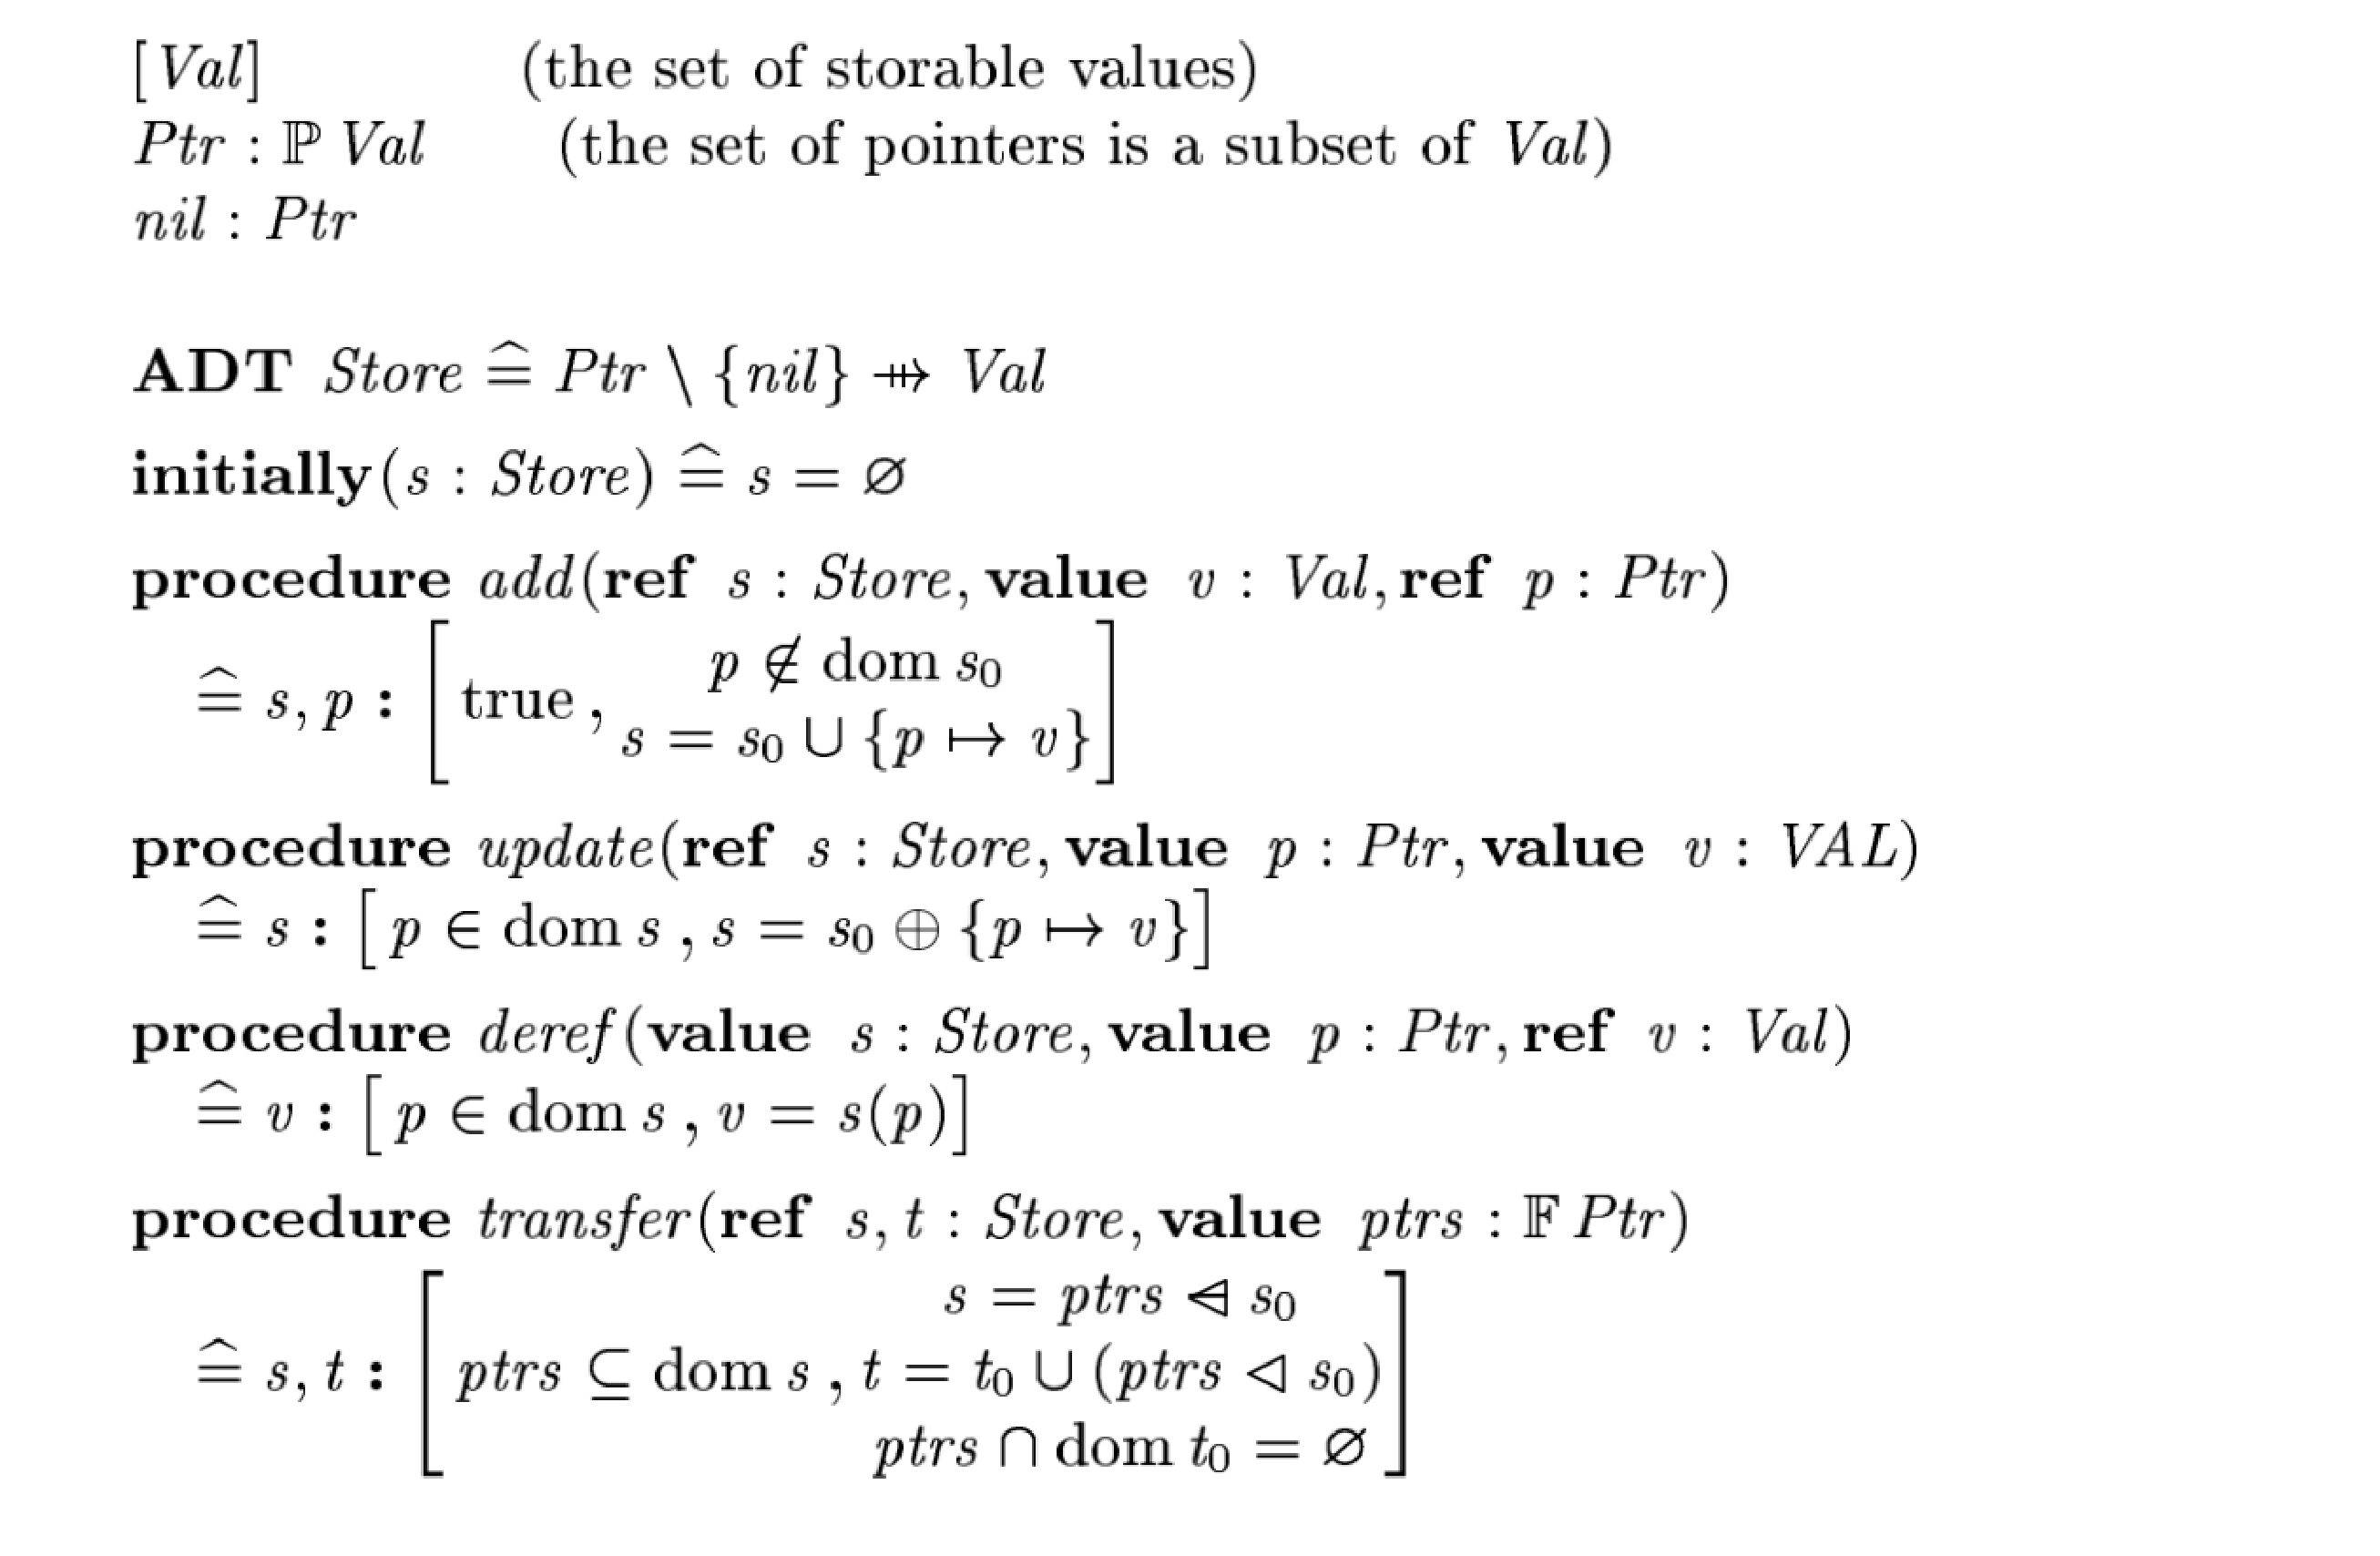
\includegraphics[width=0.5\textwidth]{LocalStoreADT.pdf}
\Description{Z specification for Local Store ADT}
\caption{Z specification for Local Store ADT, from
  \citet{utting1995,utting1998}}
\label{fig1}
\end{figure}

The ADT has five methods:
\begin{itemize}
\item \textbf{add} in a new pointer to value mapping.
\item \textbf{update} an existing mapping
\item \textbf{deref}erence a pointer, returning the corresponding
  value.
\item \textbf{transfer} a pointer from one store into another.
\end{itemize}

We could convert the Z ADT to Dafny quite straightforwardly (see
Figure~\ref{fig2}) but unfortunately this can't really be used to
emulate local stores.  To see why, consider the signature of the
``\textbf{deref}'' method. This returns the dereferenced value of
``$v$'' --- however Dafny doesn't make it possible to place any
further restrictions on the use -- the result is no longer tied to the
local store in any way.

\begin{figure}[htb]
\centering
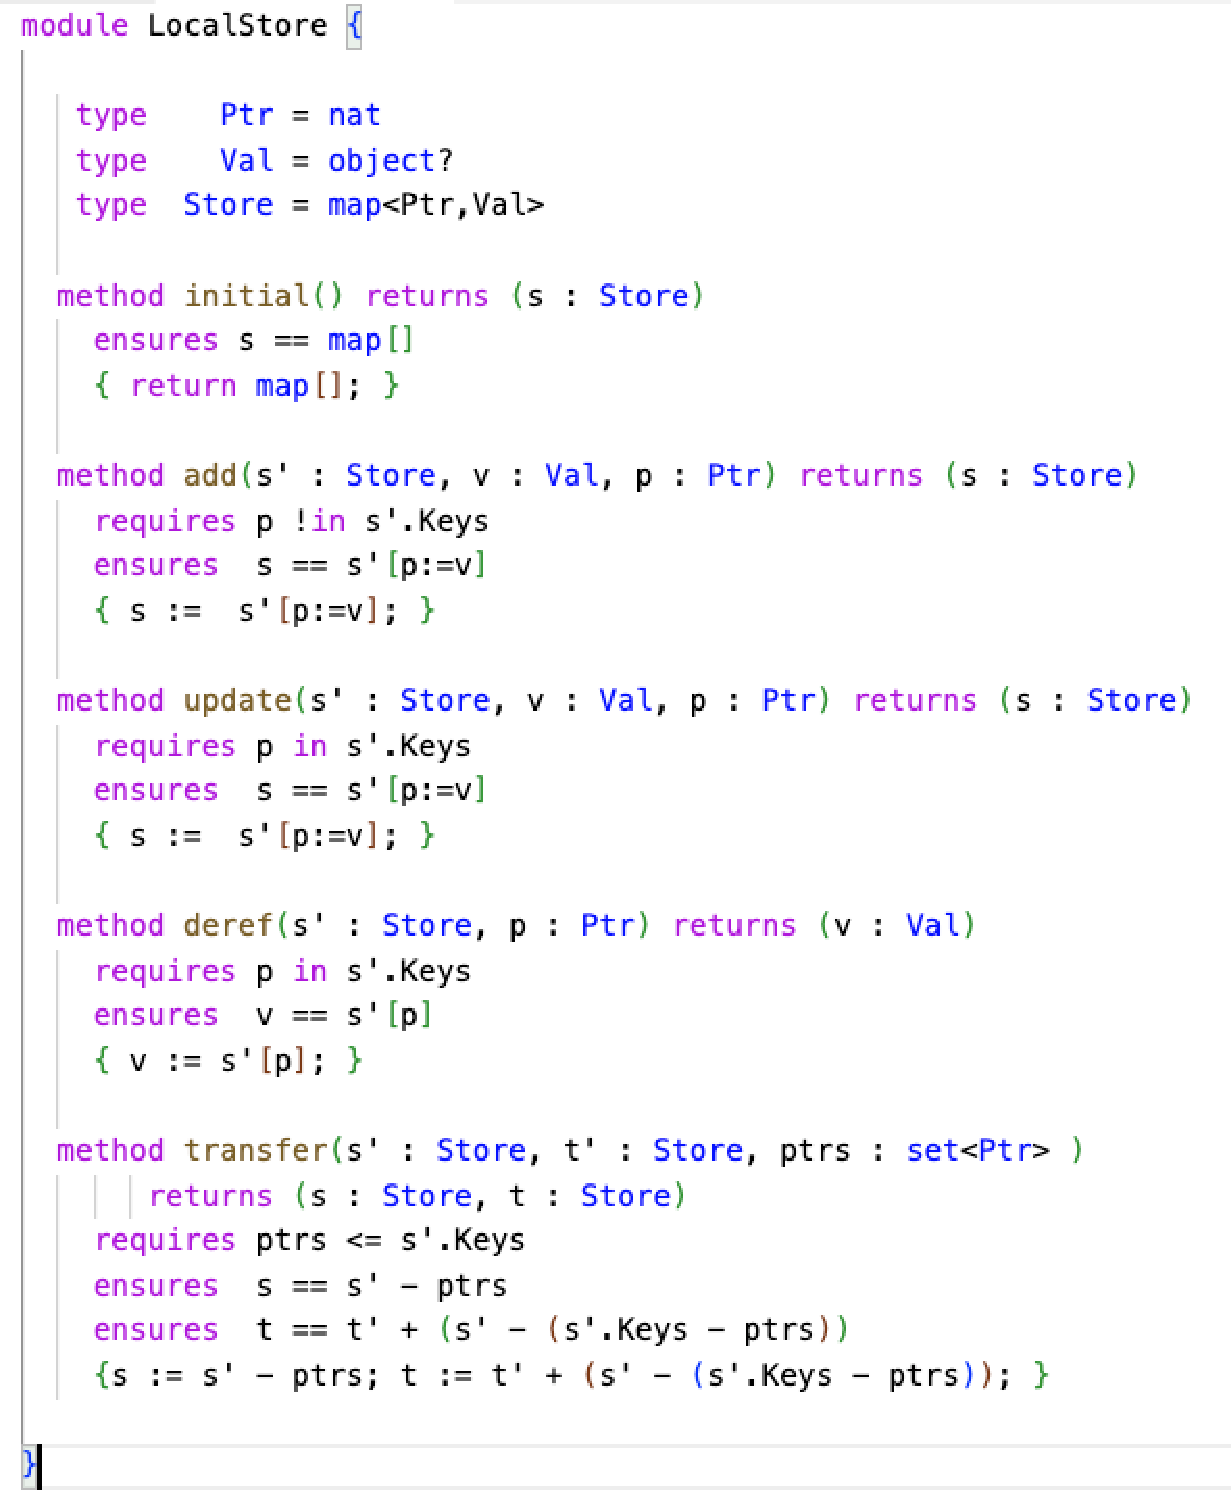
\includegraphics[width=0.5\textwidth]{LocalStoreDafny.pdf}
\Description{Dafny Local Store ADT}
\caption{Dafny Local Store ADT}
\label{fig2}
\end{figure}




\subsection{Local Stores and Objects}

Based on our work-in-progress of models of ownership in
programming languages \cite{dafnydala-ftfjp2024}, we surmised the
problem was that the Dafny objects in the store were not tied tightly
enough to the store to which they belonged. 

The core of our ownership model is the Dafny class \lstinline+Object+
(note that while \lstinline+object+ is a reserved word in Dafny,
\lstinline+Object+ is not --- neither is \lstinline+Class+)). We will
reuse the design of class Object \lstinline+Object+ to model an object
allocated in a local store. In particular, we have an
``\lstinline+owner+'' field in \lstinline+Object+ which holds the
local store in which the object is allocated -- set up when the Object
is allocated.

\begin{lstlisting}
  class Object {  
      const owner : Store
 
    constructor(oo : Store) 
      ensures  owner  == oo
      { 
        owner := r; 
        ...
\end{lstlisting}

Programmers must ensure objects they wish to use in local stores
are instances of classes that extend our \lstinline+Object+,
rather than Dafny's \lstinline+object+. Once that's done
they can use Dafny assertions to constrain object references
to refer only to instances within a particular store, or the same
store as some other object.  Consider the following example:

\begin{lstlisting}
  method disjoint(a : Object, b : Object)
     requires a.owner != b.owner
     modifies a`counter
     ensures  a.counter >  old(a.counter)
     ensures  b.counter == old(b.counter)
     {
       a.thump();
      }
\end{lstlisting}

\noindent here, the two arguments a and b are in two different local stores 
they must be two different objects. As a result, if a is modified,
we can still establish that b is not modified: both postconditions can
be verified.  Without the precondition saying the owning local stores
are disjoint, the postcondition ensuring that \lstinline+b.counter+  is
unchanged even though  \lstinline+a.counter+ most certainly is changed
could not be verified.

The result is not that dissimilar to programming in a
language with explicit region allocation: we can allocate a store,
then allocate objects with the store, then use those objects.

\begin{lstlisting}
  method Main()
     {
       var global : Store = new Store();
       ...
       while (stream.notEmpty)
       {
         var local : Store = new Store();
         process(stream.current, within:=local);
         stream.advance();
       }
     }
\end{lstlisting}

The catch is that, unlike e.g.\ Rust, Euler, Cyclone, or Linear Dafny,
there's no obvious way to constrain the use of the objects allocated
in the store. Although in the code above, the \lstinline+local+ store
appears to be scoped within the \lstinline+global+ store, and that
would be the case in Rust, say, our basic Dafny implementation doesn't
enforce that constraint.

\subsection{Nested Local Stores}

There are two issues that must be resolved:
\begin{itemize}
\item a nesting relationship needs to be established between stores
\item types and assertions need to be aware of that relationship
\end{itemize}

\noindent Establishing the nesting relationship is relatively straightforward: 
we extend stores to say which other stores they are nested within,
and provide an API such \lstinline+inside(part, whole)+ that determines
if one store is inside another:

\begin{lstlisting}
    var global : Store = new Store();
    ...
    ...
    var local : Store = new Store(global);
    ...
    var localObject := new Object(local);

    assert inside(local, global); //should verify
    assert inside(global, local); //should not verify
\end{lstlisting}

While we can use the API to verify nesting relationships, we again
have to do this explicitly --- just as we have to bind instances
explicitly into a local store.  Then, objects should be constrained by
the store structure so e.g.\ a global object cannot have incoming
pointers into nested local storage.  Our programming language heap
model addresses this by implementing object fields directly in a
hashtable \cite{dafnydala-ftfjp2024}, rather than by reusing Dafny's
own fields:
\pagebreak[3]

\begin{lstlisting}
  class Object {  
      const store : Store;
      var fields : map<string,Object>;  
\end{lstlisting}

Using this, we can e.g. place constraints on which references are
permitted:


\begin{lstlisting}
    predicate AllOutgoingRefsDala()
      reads this`fields
        { forall n <- fields ::
            DalaRefOK(kind, fields[n].kind) }
\end{lstlisting}

To gain maximum advantage of local stores, either some kind of
reflexive access to object's fields would be required, or a Dafny
plugin could be written to extend the compiler to undertake the
checks. Again referring back to Euler, a plugin to implement the
rule that stores may not be components of other stores, and may only
be passed as var parameters (i.e. only up the stack,  but not returned
down it should be straightforward. Establishing proof obligations
that an object can only be accessed when it's store is in scope
appears no harder in principle than ensuring that keys must be in a
Dafny map before they can be accessed. 


\subsection{From Stores to Owners}

Dynamic Frames, like desmesnes before them, require objects e.g. to
delineate their representations for framing, typically by writing a
function (desmesnes \cite{wills91} or original dynamic frames
\cite{dynamic-frames-fm2006}, or by updating a data structure
explicitly --- Dafny's \lstinline+Repr+ is a field, not a function.
For example, a lookup table implemented by two parallel arrays
would need to set \lstinline+Repr+ explicitly in its constructor:

\begin{lstlisting}
class Table<Data> {
  ghost var Repr: set<object>

  var keys : array<int>
  var values : array<Option<Data>>

  var size : nat
  var capacity : nat
    
  constructor (initial : nat)
    requires initial > 0
    ensures Valid() && fresh(Repr)
    {   
       capacity := initial;
       new;
       keys := new int[capacity];
       values := new Option<Data>[capacity](_ => None);

       size := 0;
       Repr := { this, keys, values };
     }
 
\end{lstlisting}


\noindent and then update \lstinline+Repr+
after every method that changes the representation:

\begin{lstlisting}
method Expand()
    requires Valid()
    modifies this`keys, this`values, this`capacity, this`Repr
    ensures Valid() && fresh(Repr - old(Repr))
    ensures size == old(size)
    ensures capacity == old(capacity) * 2
   {
       keys := new int[capacity * 2] //...
       values := new Option<Data>[capacity * 2] //...
       capacity := capacity * 2;

       Repr := { this, keys, values }; 
\end{lstlisting}


\noindent In contrast, a desmesnes function would only need to be
defined once, and could just be called whenever the footprint of the
representation needed to be determined:

\begin{lstlisting}
function desmesnes() : set<object> {{this,keys,values}} 
\end{lstlisting}


We hypothesize that ownership offered by local stores can reduce the
effort further: rather than defining either a \lstinline+Repr+ data
structure or a desmesnes function, programmers could simply allocate
an object's representation within a local store for that purpose:

\begin{lstlisting}
class Table<Data> {
  ghost var Repr: Store

  var keys : array<int>
  var values : array<Option<Data>>

  var size : nat
  var capacity : nat
    
  constructor (initial : nat)
    requires initial > 0
    ensures Valid()
    {  
       const ReprStore := new Store(this);
      
       capacity := initial;
       new;
       keys := new array<int>(capacity, ReprStore);
       values := new Option<Data>(capacity, ReprStore);

       size := 0;
     }
 
\end{lstlisting}

\noindent or one step further, providing every object with a store,
and allowing types or variables to be annotated, we could arrive at
something much close to Ownership Types \cite{noble_flexible_1998} or Rust:

\begin{lstlisting}
class Table<Data> {
  var {:rep}  keys : array<int>
  var {:rep} values : array<Option<Data>>

  var size : nat
  var capacity : nat
    
  constructor (initial : nat)
    requires initial > 0
    ensures Valid()
    {  
       capacity := initial;
       new;
       keys := new {:rep} array<int>(capacity);
       values := new {:rep} Option<Data>(capacity);

       size := 0;
     }
 
\end{lstlisting}





%% we have shown how
%% Dafny's object model can be extended to incorporate local stores into
%% object implementations, and how we can use those local stores to
%% support reasoning about aliasing.


%% The key fields of an \lstinline+Object+ are the \lstinline+kind+,
%% the \lstinline+fieldKinds+, and the object's \lstinline+fields+.

%% The Dala model is fundamentally untyped, in that it is not set up to track e.g.\ the differences between a Point and a Rectangle class. Rather the 
%% \lstinline+kind+ field captures the object's ownership capability: \
%% Immutable (\lstinline+Imm+),
%% Isolated (\lstinline+Iso+),
%% or Local (\lstinline+Mut+, originally mutable).

%% \begin{lstlisting}
%%     datatype Kind = Imm | Iso | Mut 
%% \end{lstlisting}

%% We treat Dala's ownership capabilities more like meta-types rather that traditional types:
%% they are close to what are often called
%% "reference capabilities"~\cite{caps-ecoop2001,castegren_reference_2016} but 
%% apply to individual objects, rather than each reference to an object.
%% In many languages capabilities manifest as additional keywords or attributes attached to variables that control how those variables may be used --- i.e.\ how they relate to heap topologies and their evolution. In the Dafny code example above, the difference between \lstinline+const+ and \lstinline+var+ could potentially be considered different kinds of reference capability.

%% In Dala, then, an object's \lstinline+kind+ is the kind (ownership capability) of that object. The \lstinline+fields+ map models object' fields as a map between field names ( strings) and the \lstinline+Object+s stored in each field; the \lstinline+fieldKinds+ map likewise gives the declared kind for each field.

%% Dafny \lstinline+map+s are immutable --- only Dafny \lstinline+class+ instances are mutable: only \lstinline+var+ fields of classes; \lstinline+const+ fields are, well, constant.  What this means is that while the values stored by Dala objects' fields can change (or rather, while our model permits them to change) the kinds of each field of each instance of that Dahlia class are fixed.

%% The \lstinline+Object+ class contains a number of helper functions, such as \lstinline+outgoing()+, which returns all outgoing references from an object, abstracting away field names; and \lstinline+fieldNames()+ which returns the names of fields, without their values. 

%% Finally, the class contains a Dafny invariant, represented as a Dafny predicate conventionally called \lstinline+Valid()+, which ensures the validity of each individual object.  This predicate is typically defined as a conjunction of smaller invariants that must usually be adjusted to suit the particular heap being modelled. A minimal validity predicate would be something like this: 

%% \begin{lstlisting}
%%     predicate Valid()
%%     reads this`fields
%%       {  AllFieldsAreDeclared() 
%%         && AllFieldsConsistentWithDclrn() }
%% \end{lstlisting}

%% \noindent saying that all fields (entries in the \lstinline+fields+) must have a corresponding entry in the \lstinline+fieldKinds+, and that the kind of object stored in a field must match the kind expected for that field.  These are defined by auxiliary predicates: 

%% \begin{lstlisting}
%%     predicate AllFieldsAreDeclared() 
%%       reads this`fields 
%%         { fields.Keys <=set  fieldKinds.Keys }

%%     predicate AllFieldsConsistentWithDclrn() 
%%       requires AllFieldsAreDeclared()
%%       reads this`fields 
%%         { forall n <- fields ::
%%             fieldKinds[n] == fields[n].kind }
%% \end{lstlisting}



%% \subsection{Dala Heaps}

%% The other main structure in Dala is the heap itself, modelled by the eponymous \lstinline+Heap+ class. The Heap class looks trivial --- a Dala heap is just a set of Dala objects:

%% \begin{lstlisting}
%% class Heap {
%%   var objects : set<Object>
%% \end{lstlisting}

%%  \noindent The full Heap class contains many auxiliary functions and invariants to capture the non-local structure of the heap. Thus there are corresponding class invariant validity predicates:

%% \begin{lstlisting}
%%     predicate Valid() 
%%       reads this`objects, objects
%%         { ObjectsAreValid(objects)
%%           && OutgoingRefsInThisHeap(objects) }
%% \end{lstlisting}

%% \noindent where \lstinline+ObjectsAreValid(objects)+  asserts each object's own \lstinline+Valid()+ predicate; and \lstinline+OutgoingRefsInThisHeap+ checks that the heap is closed, in the sense that there are no references to objects somehow "outside" the heap:

%% \begin{lstlisting}
%% predicate ObjectsAreValid(os : set<Object>) 
%%   reads os
%%     { (forall o <- os :: o.Valid()) }
        
%% predicate OutgoingRefsInThisHeap(os : set<Object>) 
%%   reads this`objects, objects, os
%%     { (forall o <- os :: o.outgoing() <=set objects) }
%% \end{lstlisting}

%% \noindent The validity predicate will typically be invoked in method preconditions --- Dafny does not assert class invariants automatically, rather programmers must follow conventions~\cite{Parkinson07}.

%% Unlike individual objects, Dala models often need to control the evolution of the heap, and so the class also declares an additional "two-state" predicate to capture the history constraint~\cite{Leavens-etal07}. Unlike normal (aka "one-state") predicates, two-state predicates have access both to current values (unmarked) and values at the start of the containing method call (marked "\lstinline+old+"). As such, two-state predicates can only be invoked from "two-state contexts", such as within an \lstinline+ensures+ clause or an assertion in a method body, 
%% where there are two states that can be compared.


%% %% reveal removed from example...
%% \begin{lstlisting}
%%     twostate predicate Valid2()
%%       reads this`objects, objects, objects`fields
%%       ensures Valid2() ==> Valid()
%%         { Valid() && HeapObjectsAreMonotonic() }
%% \end{lstlisting}










%% Here, for example, we can require that heap objects are monotonic --- i.e that objects are never actually removed from the heap. (Note that heap models that e.g.\ wish to model explicit memory deallocation probably would not include this invariant).

%% \begin{lstlisting}
%%     twostate predicate HeapObjectsAreMonotonic() 
%%       reads this`objects
%%         { old(objects) <=set objects }
%% \end{lstlisting}


%% Other  utility functions are then provided as methods outside the class. For example: \lstinline+edges(objects)+ transforms a set of objects --- often the \lstinline+objects+ field of a heap --- into an adjacency set, i.e.\ a set of $(\textit{from},\textit{name},\textit{to})$ 
%% triples as an alternative representation of the whole graph.
%% Due to the idiosyncrasies of Dafny's verification, it turned out easier to generate the edge-list representation from the set-of-objects representation, rather than the other way around, or by maintaining both representations and continually assuring an overanxious Dafny, at pretty much every line of code, that the two were in sync.



%% \subsection{Dala Ownership Hierarchy}

%% We need to encode the ownership capability hierarchy as a Dafny predicate, that determines whether an object of kind \lstinline+f+ (from) can point to an object of kind \lstinline+t+ (to).  (Note Dafny's alternative prefix syntax for repeated Boolean conjunctions.)

%% %\pagebreak

%% \begin{lstlisting}
%%     predicate DalaRefOK(f : Kind, t : Kind)
%%       {
%%         || t.Imm?                   //anything can point to Imm
%%         || f.Mut?                   //mut can point to anything   
%%         || (f.Iso? && t.Iso?)       //iso can point to Iso
%%       }
%% \end{lstlisting}

%% Finally we need to work this constraint throughout the heap model as a whole. We expand on the Object class invariant to ensure that all the field values --- the outgoing references --- confirm to the Dala model:

%% \begin{lstlisting}
%%     predicate Valid()
%%       reads this`fields
%%         {
%%         && AllFieldsAreDeclared()
%%         && AllFieldsConsistentWithDclrn()
%%         && AllOutgoingRefsDala()
%%         }
%% \end{lstlisting}

%% \noindent based on an auxiliary predicate that quantifies over all the fields in the object, and requires that the object's \lstinline+kind+ is compatible with the kind of the contents of each field \lstinline+fields[n].kind+:

%% \begin{lstlisting}
%%     predicate AllOutgoingRefsDala()
%%       reads this`fields
%%         { forall n <- fields ::
%%             DalaRefOK(kind, fields[n].kind) }
%% \end{lstlisting}



%% \subsection{Modelling Operations}

%% Given we are taking a lightweight approach, we do not wish to produce a full operational semantics for Dala
%% (or, likewise, require that programmers would have to be able to read a complete semantics for a language e.g.\ to find out what an "immutable" or a "unique" object means).  Rather, we model the interface between the operational semantics or an interpreter as a series of Dafny methods on the \lstinline+Heap+ class. The code of these methods are trivial: the tricks come in writing the necessary pre- and post-conditions so that Dafny can verify that they maintain the invariants structuring the heap, i.e.\ the predicates installed as the one-state class invariant \lstinline+Valid()+  and two-state history constraint \lstinline+Valid2()+ defined within the Heap class.
%% Table~\ref{tab1} on the following page shows the core operations we modelled to capture basic heap semantics


%% For example, here is the code of the interface method for adding a new object within the heap:

%% \begin{lstlisting}
%%     method  fAddObject(nu : Object)
%%       { objects := objects + {nu}; }
%% \end{lstlisting}

%% \noindent so far so good: add the \lstinline+nu+ object into the set of objects on the heap. Dafny abstracts methods as their pre-conditions (\lstinline+requires+) and post-conditions (\lstinline+ensures+) so the actual method header must include these specifications:

%% \begin{lstlisting}
%%     method  fAddObject(nu : Object)
%%         requires Valid()
%%         requires nu.Valid()
%%         requires nu.size() == 0
%%         requires nu !in objects
%%         modifies this`objects
%%         ensures Valid2()
%%         ensures unchanged(nu)
%%         ensures objects == old(objects) + {nu};
%% \end{lstlisting}

%% \noindent so that the method can rely on the class invariants of both heap and new object; check that the new object has no fields (to which objects would they refer?); that the new object isn't already in the heap; that it will modify the list of objects in the heap; and that when completed the history constraint will be maintained (which also maintains the class invariant); that the new object itself is not modified; and that the objects in the heap now consist of all the objects previously in the heap, plus the object just added!\footnote{Whew!}.  We list these here not because the details are really important --- they're not --- but rather to give an idea of the amount of effort required to specify something that simple. 

%% Finally, \lstinline+fAddObject+ requires another three lines within the method body to enable Dafny to verify the invariants:

%% \begin{lstlisting}
%%     assert edges(objects)
%%     == edges(objects + {nu})
%%     == old(edges(objects));
%% \end{lstlisting}

%% \noindent The issue here is that Dafny's axioms for the built-in collections (here sets) do not cover extensionality:  this assertion provides a hint to the verifier that adding an object with no outgoing edges doesn't change the edges in the heap. 


%% \begin{table*}[hbtp]
%%     \caption{Core API for basic Dala model.}
%%     \label{tab1}
%% % \begin{center}
%% % \mbox{
%% \begin{flushleft}
%% \ \ \ \ \ \ \ \ \ \ \daf{\dkw{method}  fAddObject(nu : Object)} --- add a new object to the heap.\\
%% \ \ \ \ \ \ \ \ \ \ \daf{\dkw{predicate} fExists(o : Object, n : string)} --- true if field f has a value (is not null)\\
%% \ \ \ \ \ \ \ \ \ \ \daf{\dkw{function} fRead(o : Object, n : string) : (r : Object)} --- read field value\\
%% \ \ \ \ \ \ \ \ \ \ \daf{\dkw{method} fInitialise(o : Object, f : string, t : Object)} --- initialise a null field\\
%% \ \ \ \ \ \ \ \ \ \ \daf{\dkw{method} fNullify(o : Object, f : string)} --- remove a field value\\
%% ~ \\
%% \ \ \ \ \ \ \ \ \ \ \daf{\dkw{method}  dynMove(o : Object, n : string, f : Object, m : string)\\
%% \ \ \ \ \ \ \ \ \ \ \ \ \dkw{returns} (r : Status)} --- Dala dynamically checked "move" \daf{o.n <- f.m;}\\
%% \ \ \ \ \ \ \ \ \ \ \daf{\dkw{method} dynCopy(o : Object, n : string, f : Object, m : string)\\
%% \ \ \ \ \ \ \ \ \ \ \ \ \dkw{returns} (r : Status)} --- Dala dynamically checked "copy" \daf{o.n := f.m;}
%% \end{flushleft}
%% % }
%% % \end{center}
%% \end{table*}







%% Then, perhaps surprisingly, we need only a few additional annotations for Dafny to be able to verify that the operations of the language maintain the heap structures so that the ownership capability hierarchy is preserved. Much of the work is done by \lstinline+fInitialise+, which writes a  value into a waiting empty field --- 
%% in fact, really by only three preconditions (or really by two actual preconditions and the invariant) of \lstinline+fInitialise+:

%% \begin{lstlisting}
%%     method {:timeLimit 60}
%%       fInitialise(o : Object, f : string, t : Object) 
%%         requires Valid()
%%         requires o.fieldKinds[f] == t.kind
%%         requires DalaRefOK(o.kind,t.kind)
%%         ...
%%       {
%% \end{lstlisting}

%% The first precondition is just the class invariant (that's the precondition that was already there).  By extending the the class invariant to include \lstinline+DalaRefOK+, Dafny automatically assumes the object capability hierarchy will be maintained upon entry to the method; and because it is also incorporated in the history constraint in the postcondition, the method itself must also maintain the hierarchy.  The second precondition requires than  object about to be assigned to a field is the kind of the object expected by that field (Dala kinds are non-polymorphic and invariant). The third precondition requires that a references from the source object to the target will also maintain the object capability hierarchy.   So we have that the existing references maintain the  hierarchy in the pre-state; now the new reference also maintains the hierarchy; so all the references in the heap maintain the hierarchy in the post-state and initialise verifies.










%% \subsection{Immutability}

%% Many programming languages support one kind or another of immutable objects (also known as value objects, frozen objects, or just values) which cannot change.  Immutability can be modelled straightforwardly in Dafny, and the predicates can be incorporated into any definition that requires immutability.
%% We will use the \lstinline+kind+s of objects defined above to distinguish between immutable vs mutable objects.
%% Then we must give some semantics to the \lstinline+Imm+ kind of immutable objects. What makes an object immutable is that "naught changeth thee"~\cite{immortalinvisible}, i.e.\ that the object is the same before any interaction as it is afterwards.  We can encode this as a two-state predicate, conjoined into a heap's \lstinline+Valid2()+ predicate:

%% \begin{lstlisting}
%% twostate predicate AllImmutablesAreImmutable() 
%%   reads this`objects, objects, objects`fields
%%     {
%%       forall o <- (objects * old(objects)) :: 
%%         o.kind.Imm? ==> (o.fields == old(o.fields))
%%     }
%% \end{lstlisting}

%% \noindent which means for all objects existing both in the pre- and post-states, if an object's kind is immutable, then all its fields in the \lstinline+old+ pre-state must equal those in the current post-state. Note that since Dafny maps are themselves immutable values, we can compare entire maps to one another with simple equality.

%% \subsection{Uniqueness}

%% Another feature enjoyed by many of the coming generation of imperative languages is uniqueness: that there is at most one reference to any unique object~\cite{Islands}. This is also relatively straightforward to model in Dafny,
%% and so supports Dala's  unique objects --- mostly known as Isolated Objects, or Isolates, thus kind \lstinline+Iso+.
%% We need to express the invariant that a unique Iso object has no more than one incoming reference. We can write an auxiliary function to extract all the (should-be) unique-kind objects --- of note are three postconditions that were required to facilitate verification: that every object in the result is an Iso; that all the Isos in the input are in the output; and that if the input is empty, so is the output.

%% \begin{lstlisting}
%%   function justTheIsos(os : set<Object>) : (rs : set<Object>) 
%%       reads os
%%       ensures forall r <- rs :: r.kind.Iso?
%%       ensures forall o <- os :: o.kind.Iso? ==> o in rs
%%       ensures (os == {}) ==> (rs == {})
%%         {
%%           set o <- os | o.kind.Iso?
%%         }  
%%     \end{lstlisting}

%% Using this function, and a function of the same complexity that
%% calculates an object's reference count (given an object \lstinline+i+ and set of
%% edges \lstinline+edges+ it counts edges incident on \lstinline+i+) 
%% we can  define an invariant that all  Isos have no more than one incoming reference:

%% \begin{lstlisting}
%%     predicate IsosAreUnique(os : set<Object>)
%%     reads os
%%       {
%%         var edges := edges(os);
%%         var isos := justTheIsos(os);
%%         forall i <- isos :: refCntEdges(i, edges) <= 1
%%       } 
%% \end{lstlisting}

%% This is the easy part. The harder part is that every operation that might modify the Dala heap must be verified by Dafny, and 
%% maintaining the \lstinline+IsosAreUnique+ predicate 
%% requires several additional assertions and a lemma.  We don't have the space to go over this in detail: but here is the imperative core of the \lstinline+fInitialise+ interface method that assigns a 
%% new object to an already-null field, and the necessary additional verification assertions:

%% % \begin{lstlisting}[numbers=left,stepnumber=1,firstnumber=1]
%% %     method {:timeLimit 60} fInitialise(o : Object, f : string, t : Object) 
%% %       { 
%% %         assert t.kind.Iso? ==> refCntEdges(t,edges) == 0;
%% %         o.fields := o.fields[f := t];  
%% %         assert ObjectsAreValid({o});
%% %         assert edges(objects) == old(edges(objects)) + {Edge(o,f,t)};
%% %         assert (o != t) ==> incomingEdges(t,{Edge(t,f,o)}) != {Edge(o,f,t)};
%% %         assert incomingEdges(t,{Edge(o,f,t)}) == {Edge(o,f,t)};
%% %         RefCountDistOverDisjointEdges(justTheIsos(edges), old(edges), {Edge(o,f,t)});
%% %       }
%% % \end{lstlisting}
%% %
%% % \noindent Note in particular:\\
%% % \noindent line 1, \lstinline+{:timeLimit 60}+ tells Dafny to spend more time to verify this method;\\
%% % \noindent line 3 we reassure Dafny that if the new field value is supposed to be unique, then  it currently has no incoming references from other fields.
%% % (If the object has just been read from a field, that field must already have been nullified, thus dropping the reference);
%% % This assertion acts as a hint to the verifier.\\
%% % \noindent line 4 does all the work that needs to be done;\\
%% % \noindent line 5 reminds Dafny that all objects should still be valid individually;\\
%% % \noindent line 6 tells Dafny how the edges in the heap graph have changed as a result of line 4;\\
%% % \noindent lines 7 \& 8 explain consequences of the changes made in line 4 \& described in 6;\\
%% % \noindent finally, line 9 invokes a lemma expressing the graph-theoretic property that the reference counts to a set of objects 
%% % distributes over two disjoint sets of edges involving those objects.


%% \begin{lstlisting}[numbers=left,stepnumber=1,firstnumber=1,xleftmargin=5mm]
%% method {:timeLimit 60}
%% fInitialise(o : Object, f : string, t : Object) 
%% { 
%% assert t.kind.Iso? ==> refCntEdges(t,edges) == 0;
%% o.fields := o.fields[f := t];  
%% assert ObjectsAreValid({o});
%% assert edges(objects)
%%        == old(edges(objects)) + {Edge(o,f,t)};
%% assert (o != t) ==>
%%  incomingEdges(t,{Edge(t,f,o)}) != {Edge(o,f,t)};
%% assert incomingEdges(t,{Edge(o,f,t)})
%%     == {Edge(o,f,t)};
%% RefCountDistOverDisjointEdges(justTheIsos(edges), 
%%   old(edges), {Edge(o,f,t)});
%% }
%% \end{lstlisting}

%% \noindent Note in particular:\\
%% \noindent line 1 \lstinline+{:timeLimit 60}+ tells Dafny to work harder on this method;\\
%% \noindent line 4 reassures Dafny that if the new field value is supposed to be unique,   it currently has no incoming references from other fields.
%% (If the object has just been read from a field, that field must already have been nullified, thus dropping the reference);
%% This assertion acts as a hint to the verifier.\\
%% \noindent line 5 does all the work that needs to be done;\\
%% \noindent line 6 hints to Dafny that each individual object should still be valid;\\
%% \noindent lines 7 \& 8  tell Dafny how the edges in the heap should have changed as a result of line 5;\\
%% \noindent lines 9--12 explain consequences of the changes made in line 5 \& described in 7;\\
%% \noindent finally, lines 13 \& 14  invoke a lemma expressing the graph-theoretic property that the reference counts to a set of objects 
%% distributes over two disjoint sets of edges involving those objects.








%% % \section{Rust}

%% % rust stuff riped from ftdjp 2022 paper (which MUST be cited, as must MPTP)

%% % Rust~\cite{RustBook,RustPopular,MSRust} is well-known as a language that combines control of memory use, safe concurrency, and excellent compiler error messages.  Rust achieves this balance thanks to a version of \textit{ownership types}~\cite{ClaPotNobOOPSLA98,NobPotVitECOOP98,OTSurvey}
%% % (also known in the literature as ``\textit{ownership types}''
%% %~\cite{SafeRust,djpRust}) which statically track the lifetime (or owner) of each allocated object: when an object goes out of scope, all the memory owned by that object is deallocated. So far, so C$++$~\cite{cpp}, but Rust's ownership types ensure that programs remain memory safe, so very much not C$++$. 
%% % %
%% % Rust incorporates  alias burying (renamed borrowing)~\cite{borrowing} and fractional permissions~\cite{boyland:2003:fractional} to support an integral multiple-reader/single-writer concurrency model~\cite{lea98}: at any time, an object may either be accessed by multiple read-only aliases, or by a single read-write reference.

%% % Many programmers find Rust hard to learn and to use correctly~\cite{LearnRust,VizRust,HardRust,SafeRust,FightRust}.  
%% % This is because Rust's ownership types are necessarily conservative, banning not just all cprograms that are \textit{actually} unsafe, but a large number of safe programs as well. 
%% % %

%% %  One source of this complexity is the interaction between Rust's ownership and concurrency models. A multiple-reader/single-writer discipline makes sense for relatively course-grained for concurrency control, but recursively enforcing that discipline down to all inter-object references objects makes many linked structures impossible --- at least in the safe subset of Rust.     

%% \balance

%% \subsection{Move vs Copy Semantics}

%% Since 2011, C++ has distinguished between what it calls \textit{copy semantics} --- essentially the situation from earlier versions of C++, where an assignment copies memory from rvalue to lvalue, leaving both rvalue and lvalue accessible afterwards, and \textit{move semantics} where an assignment "moves" data from rvalue to lvalue,  meaning that the rvalue is conceptually nullified by the move, and so is no longer accessible~\cite{Boyland01}. (In practice, the implementation of copy and move are identical: the only difference is in the continued accessibility of the rvalue afterwards~\cite{harms_copying_1991}).
%% Rust, famously, is built around the same distinction, and Dala also uses the distinction with Isos (copying a reference to an Iso means the Iso is no longer unique, thus breaking the heap structure invariant).

%% We model both these operations. Here is the imperative core of the method that will \lstinline+move+ the contents of field \lstinline+m+ from object \lstinline+f+ into field \lstinline+n+ of object \lstinline+o+ --- we retrieve the value from the source field, nullify the destination if necessary, nullify the source, and  write the value back into the destination field.

%% \begin{lstlisting}

%%     method move(o : Object, n : string,
%%                 f : Object, m : string)
%%     {
%%       var value := f.fields[m];
%%       if (fExists(o,n)) {fNullify(o,n);}
%%       fNullify(f,m);
%%       fInitialise(o,n,value);
      
%% \end{lstlisting}

%% \noindent Verification is straightforward unless we're moving an Iso: if we are, we need to reassure Dafny that reference counts distribute over disjoint sets of edges yet again, and other similar things. 

%% Copy semantics "feels" like a more complex operation
%% than move semantics. In the physical world, copying things is certainly more complex than moving things~\cite{betabook},
%% and of course copying things paid for the development not just of personal computers but much of the supporting infrastructure (networking, laser printers, mice, Mac, Windows). In our model,  however, copying 
%% has an even simpler definition than moving, and a simpler proof that Dafny can complete automatically.  Still omitting the pre- and post-conditions, here's the entire implementation of \lstinline+copy+, not just the imperative core:

%% \hbox{
%% \begin{lstlisting}

%%     method copy(o : Object, n : string, 
%%                 f : Object, m : string)
%%     {
%%       var value := f.fields[m];
%%       if (fExists(o,n)) {fNullify(o,n);}
%%       fInitialise(o,n,value);
%% \end{lstlisting}
%% }

%% \noindent We have three of the same statements as for \lstinline+move+ --- omitting the line that nullifies the source. The pre- and post-conditions for copying are essentially the same as for moving, and the same time limit directive is required.  The key difference, it turns out, doesn't turn directly on the nullification itself, but rather on the fact that \lstinline+move+ can be used to move references to unique Iso objects, while \lstinline+copy+ cannot. Copy has a precondition that prevents it from being applied to Iso objects (by preventing it from being applied to fields whose \lstinline+fieldKind+ is Iso --- 
%% \lstinline+requires not( fieldKinds[f].Iso? )+ --- any other kind of field can never contain an Iso), so the whole question can be sidestepped, whereas move must ensure the heap structure invariants around Iso objects are maintained.

%% % \subsection{Rust: stack allocation}
 
%% % For our final example, we will sketch how stack allocation as in Rust 
%% % can be modelled in Dala~\cite{Rust}.  If our aim with earlier examples has been to show that simple things are simple,
%% % here our aim is rather to hint that complex things are possible, and to show some approaches that have proved fruitful, rather than to lay out an entire model and all the assumptions necessary to enable Dafny to verify the model. 

%% % The key difference here is that the object ownership is rather more complex. 
%% % In particular we must model a stack: objects can be allocated either on the stack and on the heap.  To model this, without running into problems with termination, we introduce another Dafny type, \lstinline+Region+: objects are owned by regions, but
%% % \lstinline+Heap+ regions are in turn owned by objects.

%% % \begin{lstlisting}
%% % datatype Region = 
%% %         Frozen
%% %       | Stack(frame : Region)  
%% %       | Frame(prev : Region, env : Object, entry : Region) 
%% %       | Heap(owner : Object)
%% % \end{lstlisting}

%% % \noindent A \lstinline+Frozen+ region is used e.g.\ to represent the bottom of  the stack (the operating system that invokes the program); 
%% % stack frames are represented by \lstinline+Frame+ objects,
%% % where \lstinline+prev+ is the preceding frame (moving down towards the bottom of the stack), and \lstinline+env+ is a \lstinline+Stack+ allocated object representing the local environment of the stack frame (local variables, arguments, etc), and \lstinline+entry+ is the "\lstinline+this+" object; while
%% % \lstinline+Stack+ marks an object allocated on the stack
%% % (compare \lstinline+Heap+) for a heap-allocated object.

%% % \vspace*{1mm}

%% % \noindent Kinds still describe the capabilities of fields of objects:

%% % \begin{lstlisting}
%% % datatype Kind = Imm | Iso | Mut | Tmp | Sus
%% % \end{lstlisting}

%% % % rust stack

%% % The key invariant about the stack is what Rust calls "no dangling references" or that "a value must outlive all its references" or
%% % "young points to old",   Ownership types call this  "no incoming references" or the "containment invariant". (This is fthe same way physics / astronomy allows us to see backwards in time towards the past, but never forwards in time, towards the future). 

%% % This is captured primarily by the \lstinline+frameOutlives+ predicate: an \textit{older} frame outlives the \textit{younger} frame if younger frame finishes executing and returns while the older frame is still running (presumably buried something further down the stack, waiting for all its younger frames to return).  We can encode this as a straightforward recursive stack traversal, as we go further down the stack, back in time, the stack grows shorter.  Dafny can determine this is structural recursion through the \lstinline+Region+ datatype: Dafny is designed so such datatype instances are always finite: so this recursion will always terminate.

%% % \begin{lstlisting}
%% % predicate frameOutlives(older : Region, younger : Region) 
%% %   requires younger.Frame?
%% %   requires older.Frame? || older.Frozen?
%% % {
%% %   (younger.prev == older) ||
%% %      (younger.prev.Frame? && frameOutlives(older, younger.prev))
%% % }
%% % \end{lstlisting}

%% % The code to manipulate the stack --- push on frames on entry, pop them off on return --- is all straightforward; the imperative core of the other operations (assignments, field reads. create object, etc) is also essentially unchanged.  The main catch is that all these methods need to assert or calculate sufficient information 
%% % for all the heap invariants to verify. A method with three or four statements can easily end up with 15-20 pre- and post-conditions combined: generally more pre-conditions than post-conditions,
%% % plus 30-40 assertions or calculations in the method to enable Dafny for validate that code.

%% % % stick staclk invaria nts 

 % local stores in Dafny
% desmesnes, regions, dynamic frames
% nested local stores
% explicit local stores vs licit ownership
%\input{loopy}
%~~~~~\section{Discussion}


\textbf{THIS REALLY NEeDS WORK OR TO BE DELETED}

\emph{
it's from the SWEN324 paper, basically, it tlaks about courses not programming.
%
what needs to happen is write some crap in here a bout frameworks \ldots
%
can have some reflection on Dafny I guess
%
}
\begin{verbatim}
TOPICS:
 1. evolving a ftamework in Dafny
    (not currenly using Dafny modules or refinement)
 2. 
 3. 
\end{verbatim}



Mathematics may still be taught via pencil and paper (or \LaTeX) but
these days teaching programming is impossible without a toolchain: a
language implementation, a development environment, and the other
accoutrements students expect.  Our course design teaches verification
as a specially intense kind of programming (``More programming than
programming is our motto'' \cite{bladeRunnerFilm}) --- this requires
a toolchain that is reliable, scalable, and supported enough to cope
with daily use by hundreds of students.
%
Luckily, we found the current versions Dafny were certainly good
enough for our purposes: we were able to spend the vast majority of
our efforts in teaching the practices and principles of verification,
rather than working around problems and bugs in the tools. While we
encountered roughly one serious bug during each course offering so
far, the Dafny project team resolved them assiduously.Our overall
experience with Dafny was very positive. 

Probably the biggest issue we
encountered was just finding the resources -- notably staff time and
effort --- to support rapid feedback via automated marking of the
weekly questions and the assignments. The problem was not so much the
necessary infrastructure, which is essentially a one-off cost, but the
advance preparation needed for automated marking of every assignment.
Basically, marking must be complete before an assignment can be
released, rendering it no longer possible to write underspecified assignments
which point students in a general direction, wait until the assignment deadline, and then take as much
time as necessary \textit{after the students have submitted their work}
to work out the marks, the desired solutions, or
even \textit{whether solutions are possible}. All this work must now be completed beforehand.

\vspace*{5mm}

That said, we did strike three more technical issues that could be
addressed via changes to Dafny's design:

\paragraph{Program Testing:}  We encourage students to start by testing
their implementations, because it is easier to verify code that is
correct
% against specifications that are also correct
than it is to
verify incorrect code :-).
%
Dafny’s tight integration of proving and programming unfortunately
means that programs cannot easily be tested until they are fully verified.
We observed students continually “commenting out” assertions and
preconditions to be able to test their programs, and then undoing
those comments to undertake verification. There are four related problems here.

First, Dafny's requirements to prove all memory accesses safe,
and that all programs terminate, often mean even simple programs
have to be heavily annotated just to compile.
A method to swap two array elements will require 
array reads and writes to be in bounds;
the obvious (and best practice) solution is
to define method preconditions which ensure method 
arguments are in bounds: but now all callers of the
method must themselves do enough to meet those preconditions. 

Second, while annotations, assumptions, and non-totality declarations etc.\ can be used 
to remove the need for some of these checks, they still require
students to annotate their programs explicitly, 
i.e.\ so students always have to deal with the checks
even if just to tell Dafny to ignore them!

Third, while Dafny does support command line options to e.g.\ 
ignore verification and compile and run programs directly,
verification is an all-or-nothing, static affair: either
verification is attempted for the whole program, or 
all specification and verification constructs are ignored.

Fourth (and finally) the options to control verification are buried in
the command line, and are not surfaced in the Visual Studio Code IDE.

Following the example of
Gradual Dafny \cite{Figueroa2018} and Gradual Verification 
\cite{Arlt2014,Bader2018,Wise2020}
more generally should make testing easier.
Ideally students would be able to run programs in a “test mode” where
Dafny checks as many assertions, assumptions, and pre- and postconditions
as possible dynamically.  Students could then express a series of unit tests as
Dafny assertions: if the program verifies, well and good; but if not,
they would still have the option of running the program and using
print statements or host debuggers to interrogate program state.
Recent Dafny releases 
\cite{Dafny3.0.0} 
now support an 
\texttt{expect} statement that does Gradual Dafny style dynamic
checking: implementing this option may be as simple as translating
Dafny's verification condition as \texttt{expect}s rather than \texttt{assert}s. 

\paragraph{Verification Debugging:}
Much of the work of verifying Dafny programs involves students
annotating their code --- adding require and ensure clauses and
assertions until the verifier has enough information to discharge its
proof obligations.  Students find this hard because it is not obvious
what Dafny “knows” at any given program point: which assertions Dafny
is able to prove, which assertions Dafny is able to refute, and which
assertions Dafny is unable to answer (i.e. where the prover times
out). We also observed cases where Dafny is unable to verify an
assertion because it does not have enough information about variable
values --— this is particularly prevalent in code where e.g.\ 
students have forgotten to write method postconditions, or 
have not realised a particular postcondition is necessary. This
manifests as Dafny being unable to verify an assertion about a
method’s return value, and simultaneously unable to verify the
negation of that same assertion.  Even good students find this
situation intensely frustrating.  Ideally Dafny would be able to give
programmers more information about what it knows, e.g.\
by querying its underlying solver \cite{Christakis2016}.




\paragraph{Mutable Object Structure:}  Dafny is one of the few tools
that can verify programs built from composite structures of mutable
objects using class invariants and representation sets.  In practice,
this requires either explicit definitions of ``\lstinline+Valid+'' and
``\lstinline+Repr+'' attributes \cite{dafny2020} which are verbose and
complex, or implicit definitions generated via the
``\lstinline+autocontracts+'' attribute \cite{leino2013} which are
concise but opaque.  Few students were able to use either mechanism
effectively.  Perhaps by building on work verifying Rust programs,
such as Prusti \cite{Astrauskas2019} and RustBelt \cite{Jung2017}, it
should be possible to add ownership annotations to fields and
parameters, to check those annotations as with Rust's borrow checker
\cite{Markstrum2010,Dietl2011,Klabnik2019} and thus extend the
implicit definitions already generated by autocontracts.

\vspace*{5mm}

We also encountered a number of pragmatic issues that arose with Dafny, but which appear to be consequences of Dafny's design choices, and as such are less amenable to technical fixes.

\paragraph{Idiosyncrasies:}  Dafny's syntax is sometimes idiosyncratic, which students found hard to follow.  
To give just one example, here are a method and function to add two numbers:
\begin{lstlisting}
method addM (a : int, b : int) returns (c : int) { c := a + b; }
function method addF (a : int, b : int) : int { a + b }
\end{lstlisting}
The syntax for declaring the return values are different
(\lstinline+returns+ vs \lstinline+:+); the syntax for actually returning the results are different; a final semicolon is mandatory in the method and forbidden in the function. 
Adding insult to injury, methods and functions then perform very differently in the verifier:
\begin{lstlisting}[numbers=left,stepnumber=1]
     var m := addM(x,y);
     var f := addF(x,y);
     assert m == x + y;   //Fails to verify
     assert f == x + y;   //Verifies
\end{lstlisting}
Dafny verifies the assertion on line 4, because functions are incorporated into the verification context.
Dafny fails to verify the assertion on line 3, however,
because methods are always abstracted by their postconditions,
and the declaration of \lstinline+addM+ omits postconditions.
There are reasons for these choices, but they do make the language more difficult to learn.  

\paragraph{Implicit vs.\ Explicit Verification:}  We have described as taking an implicit (aka ``auto-active''  \cite{autoactive2010}) approach to verification. 
Our students, or Dafny programmers in general, 
do not construct proofs explicitly, in some verification domain that reflects on the base domain of the program: rather they
work in an extended programming language domain. 
That is, students focus on programs, and program verification, but not on the foundations of logic, programming languages, and critically, not on proof.  Our teaching practice 
builds on this implicit approach: students 
definitely need an implicit understanding of the 
underlying formal concepts --- because they
will be incapable of completing 
any work without that understanding --- but we present 
those concepts completely within the programming 
approach: we don't discuss the semantics 
of programming languages, weakest preconditions, 
the kind of inferences Dafny's underlying solver is making,
let alone how it works.
We approach software verification in
the same way that most software engineering courses 
approach statically-typed languages: students can
understand the benefits, and use the type systems,
but could not give a type-theoretic explanation
for why their programs don't compile.

Arguably the biggest weakness of this implicit approach
is that it sidesteps the question of proof.
Dafny does not illustrate proofs of programs
(other than symbolic dumps designed for debugging Dafny).
As a result, we do not expose students to formal proofs,
and in fact students never need to understand what a proof is.

We do teach that Dafny assertions can be used as ``hints'' to the verifier checker; we also show how Dafny (ghost) functions can be used within specifications or assertions to embody lemmas that Dafny cannot find itself.  In the latter part of the course, questions require (ghost) data and methods to model the state of imperative objects. We mention Dafny's \texttt{calc} statement that supports line-by-line reasoning only in passing. 

We consider this a trade-off worth making: the course stays focused on program verification, through a programming lens, 
and we use the time to allow students to complete more significant examples with more complex verification constructs,
rather than teaching proof and necessarily working on smaller examples. 



%\vfill\null
%\columnbreak

%\vspace*{1mm}
\section{Conclusion}
%\vspace*{-2mm}

In this short paper we've described our initial experience with
modelling local stores --- first class regions --- with Dafny.
Starting from an historical perspective, we've discussed how Utting's
local store ADT could be modelled in Dafny, albeit not in a way Dafny
programmers could use such an ADT effectively.

Then, drawing on our work-in-progress models of ownership in
programming languages \cite{dafnydala-ftfjp2024}, we have shown how
Dafny's object model can be extended to incorporate local stores into
object implementations, and how we can use those local stores to
support reasoning about aliasing.

On the whole we think this effort has been worthwhile: using
explicit local stores seems no more clumsy than Dafny's native dynamic
framing, and can be more precise and more flexible than the
autocontracts mechanism.  Furthermore, by providing programmers with a
notation to describe nesting relationships between local stores, we
speculate that information about such relationships may be employable
e.g.\ to generate better code for Rust or other langauges where object
lifetimes, nesting, and ownership are important.  On the other hand,
the lack of reflection in plain Dafny means that the larger prize,
tighter pelluicid integration of Dafny objects and ownership, would
require at least compiler plug-ins, or language extensions like Linear
Dafny \cite{linear-dafny-oopsla2022}.

The main disadvantage we found from using Dafny is that programmer
time to achieve verification always seems to take longer than any
estimate --- even though when working with 
Dafny, we often felt that just "one more assertion" would be enough to
verify our entire model. We consider this comes from the automatic
yet opaque style of verification that is intrinsic to Dafny. Dafny verification acts as a intermittent positive reinforcement on a variable ratio schedule, like a slot machine, with the same addictive qualities
\cite{dafny-europlop2024}.

%% sstudents get feedback
%% expectations are clear
%% can work local or remotely (COVID)
%% sthudents always nkow where they are
%% students can choose how much time and effort to invest
%% mastery means can demonstrate a ``taste'' of the topic 


% \vspace*{-1mm}

% \begin{verse}
%   \textit{
% Getting code to work is one thing.\\
% Proving it does what it's supposed to is something else.\\
% Convincing Dafny you've proved it does what it's supposed to\\
% ~~~~is something else entirely.}
% \end{verse}
% \vspace*{-10mm}
% \begin{flushright}
% ``Motto for a Software Correctness Course''\\
% Thomas J. ``Tad'' Peckish (attrib.), twitter, Oct 4 2020
% \end{flushright}


\balance
%\pagebreak 

% \section*{Data-Availability Statement}

% Dahlia is under active development.
% Low quality Dahlia models  have been submitted as additional material.
% Revised and refactored models will be submitted to ACM's artefact evaluation and archiving.

%\pagebreak

%\vspace*{1mm}
\begin{acks}
Thanks to Rustan Leino and James Wilcox, 
% and our (ex-) colleagues David Streader, Isaac Oscar Gariano, and
% Miniruwani Samarakoon for all their help with Dafny;
% to Marco Servetto for the ``marcotron'' weekly question
% system, to Royce Brown, Christo Muller, and the ECS technical staff
% for their support with the course automation; 
to Lindsay Groves, longtime custodian of Formal Methods at VUW,
to longtime collaborators Sophia Drossopoulou \& Susan Eisenbach,
to the many anonymous reviewers of slightly worse versions of related papers.
%
%This work was supported in part by the Royal Society of New Zealand Marsden Fund Grant %VUW1815 and CRP2101 and by gifts from AWS and Agoric. 
%
This work is supported in part by the Royal Society of New Zealand Te Ap\={a}rangi  Marsden Fund Te P\={u}tea Rangahau a Marsden grants VUWU1815 and CRP2101, an Amazon Research Award, and Agoric Inc.
\end{acks}

\pagebreak
%\cleardoublepage


\bibliographystyle{ACM-Reference-Format}
\bibliography{XERC-Case, XEVIL-rw, XEVIL-bibliography, XETC-biblio, XERC-verona, XERC-references, XERC-ecoop21-biblio, Xeelco-refs,  XRusty-Case, Xgrace2022, dafny}


%
\end{document}
